% Created 2017-12-09 Sat 16:39
% Intended LaTeX compiler: pdflatex
\documentclass[11pt]{article}
\usepackage[utf8]{inputenc}
\usepackage{lmodern}
\usepackage[T1]{fontenc}
\usepackage{fixltx2e}
\usepackage{graphicx}
\usepackage{longtable}
\usepackage{float}
\usepackage{wrapfig}
\usepackage{rotating}
\usepackage[normalem]{ulem}
\usepackage{amsmath}
\usepackage{textcomp}
\usepackage{marvosym}
\usepackage{wasysym}
\usepackage{amssymb}
\usepackage{amsmath}
\usepackage[version=3]{mhchem}
\usepackage[numbers,super,sort&compress]{natbib}
\usepackage{natmove}
\usepackage{url}
\usepackage{minted}
\usepackage{underscore}
\usepackage[linktocpage,pdfstartview=FitH,colorlinks,
linkcolor=blue,anchorcolor=blue,
citecolor=blue,filecolor=blue,menucolor=blue,urlcolor=blue]{hyperref}
\usepackage{attachfile}
\usepackage[left=1in, right=1in, top=1in, bottom=1in, nohead]{geometry}
\geometry{margin=1.0in}
\usepackage{hyperref}
\usepackage{amsmath}
\usepackage{graphicx}
\usepackage{epstopdf}
\usepackage{fancyhdr}
\pagestyle{fancy}
\fancyhf{}
\usepackage[labelfont=bf]{caption}
\usepackage{setspace}
\setlength{\headheight}{10.2pt}
\setlength{\headsep}{20pt}
\renewcommand{\headrulewidth}{0.5pt}
\renewcommand{\footrulewidth}{0.5pt}
\lfoot{\today}
\cfoot{\copyright\ 2016 W.\ F.\ Schneider}
\rfoot{\thepage}
\chead{\bf{Advanced Chemical Engineering Thermodynamics (CBE 60553)\vspace{12pt}}}
\lhead{\bf{Homework 8}}
\rhead{\bf{Due December 7, 2017}}
\usepackage{titlesec}
\titlespacing*{\section}
{0pt}{0.6\baselineskip}{0.2\baselineskip}
\title{University of Notre Dame\\Advanced Chemical Engineering Thermodynamics\\(CBE 60553)}
\author{Prof. William F.\ Schneider}
\usepackage{siunitx}
\usepackage[version=3]{mhchem}
\def\dbar{{\mathchar'26\mkern-12mu d}}
\setcounter{secnumdepth}{3}
\author{William F. Schneider}
\date{\today}
\title{CBE 60553 Homework}
\begin{document}

\begin{OPTIONS}
\end{OPTIONS}

\noindent \textbf{Solve each problem on separate sheets of paper, and clearly indicate the problem number and your name on each.  Carefully and neatly document your answers.  You may use a mathematical solver like Matlab or Mathematica. Use plotting software for all plots.}


\section{Partial molar concepts \label{Cp}}
\label{sec:orga95d4a6}
Following is some data on the heat evolved when 1 mole of sulfuric acid (\ce{H2SO4}) is isothermally mixed with \ce{H2O} at \SI{298}{K}.

\begin{center}
\begin{tabular}{lrrrrrrrrrr}
\hline
\(N_\ce{H2O}\) (mols) & 0.25 & 1.0 & 1.5 & 2.33 & 4.0 & 5.44 & 9.0 & 10.1 & 19.0 & 20.0\\
\(-\Delta H_\text{mix}\) (J) & 8242 & 28200 & 34980 & 44690 & 54440 & 58370 & 62800 & 64850 & 70710 & 71970\\
\hline
\end{tabular}
\end{center}

\begin{enumerate}
\item Is this mixture ideal?  Why?

\item Determine and plot the molar enthalpy of mixing as a function of mole fraction of
\ce{H2SO4}.

\item Estimate the heat evolved when \SI{100}{g} of a 60\%(w/w) sulfuric acid solution is mixed
with \SI{75}{g} of a 25\%(w/w) sulfuric acid solution.  \emph{Hints}: What is the molar
composition of the initial solutions?  Of the final one?)

\item Estimate the partial molar enthalpies of \ce{H2O} and \ce{H2SO} in a 50\%(w/w)
solution.

\item The mixing enthalpy of a ``regular'' solution can be written as \(\chi_{12}x_1x_2\).
Fit the data to this model to estimate \(\chi_{12}\) and to estimate the partial molar
enthalpies of \ce{H2O} and \ce{H2SO} in a 50\%(w/w) solution.
\end{enumerate}

\begin{center}
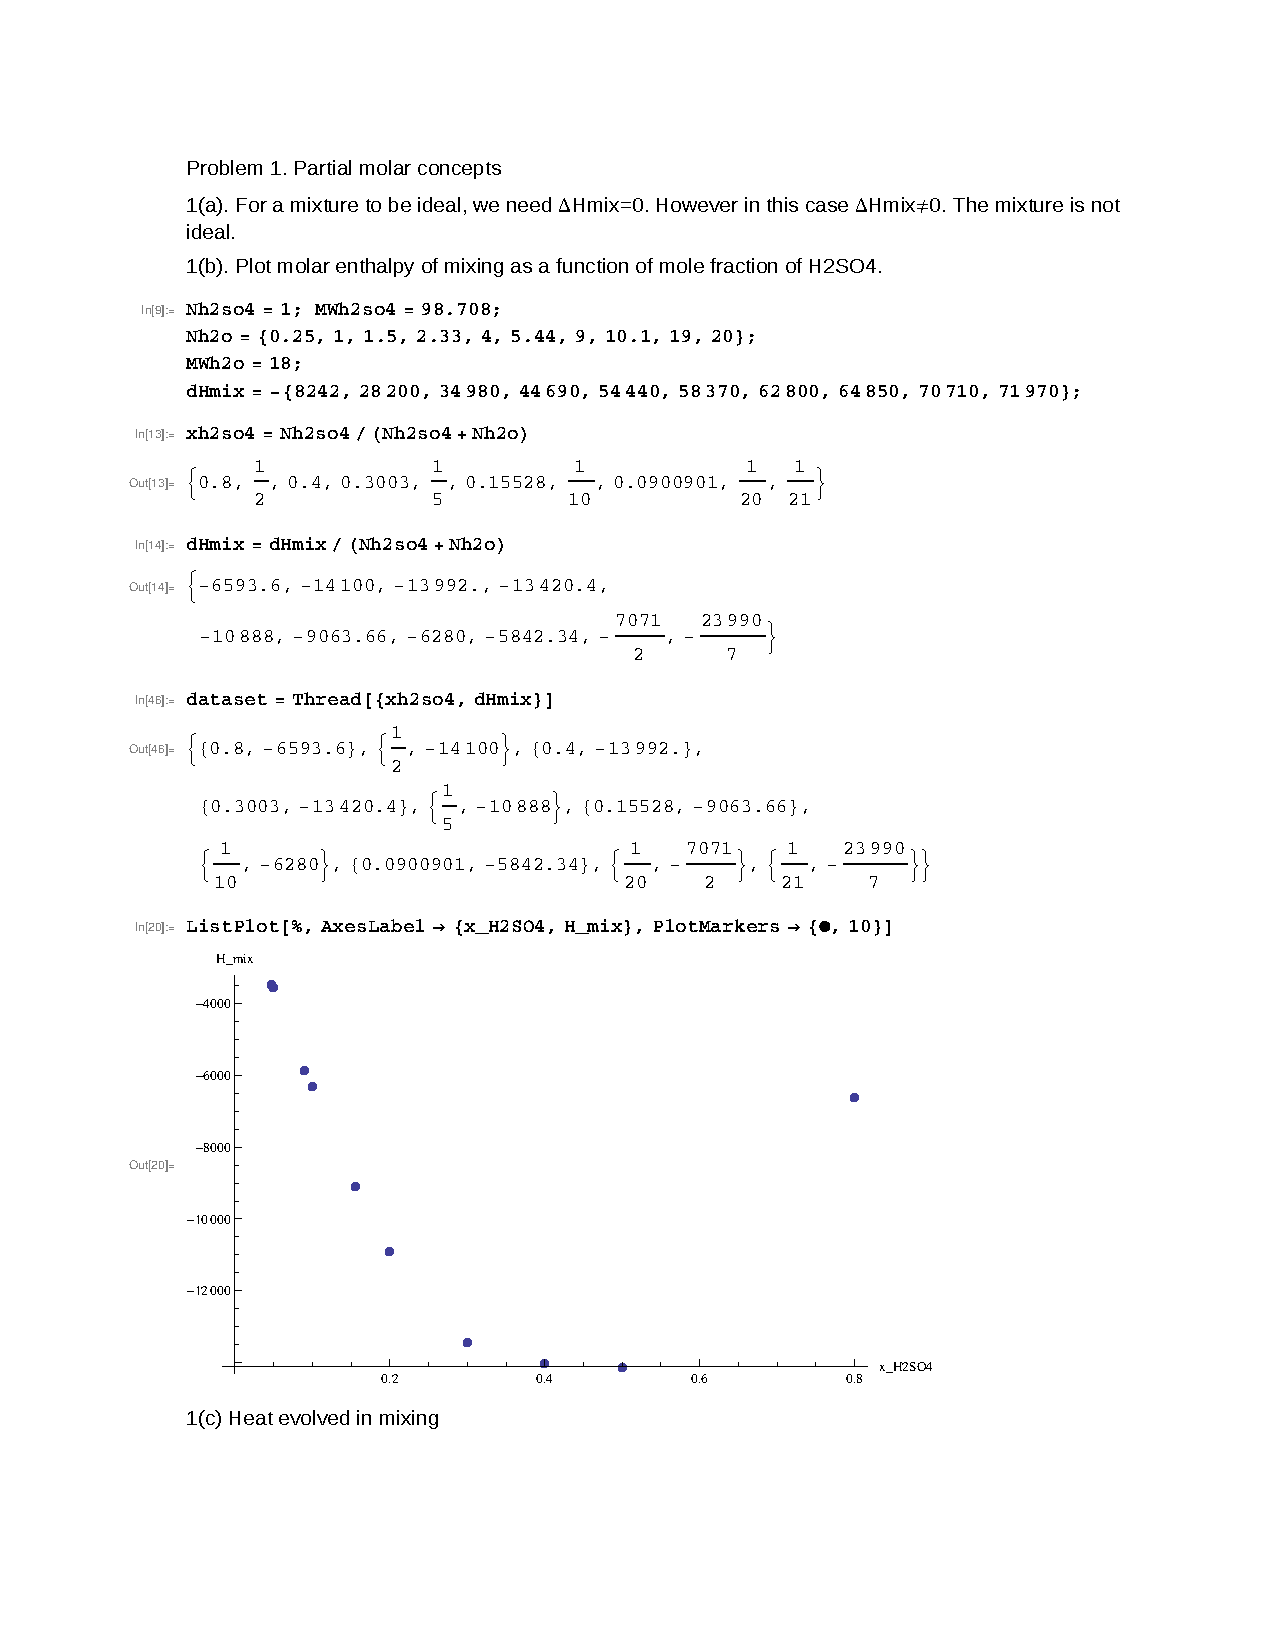
\includegraphics[width=.9\linewidth]{./HW8-Q1-soln.pdf}
\end{center}


\section{Phase diagrams for liquids \label{Cp}}
\label{sec:org3932c25}
Within the regular solution model, the free  energy of mixing two liquids is given by
\begin{equation*}
  \Delta g_\text{mix} = RT \left \{ x_\text{A} \ln x_\text{A} +  x_\text{B} \ln
    x_\text{B} +\chi_\text{AB} x_\text{A}x_\text{B} \right \}
\end{equation*}
\begin{enumerate}
\item Suppose \(\chi_\text{AB} = 5\) at 300~K for some mixture of liquids A and B.  You prepare a mixture of 0.3 mol A and 0.7 mol B at this temperature.  How many phases are
present at equilibrium, what are their compositions, and how much of each phase (if more
than one) is present?

\item What are the spinodal compositions at 300~K of the A/B mixture?

\item The binodal and spinodal curves meet at the critical point.  The second and third
derivatives of the free energy of mixing must vanish at this point.  Find the critical
composition and temperature of this mixture.  Assume that \(\chi_\text{AB} \propto 1/T\).
\end{enumerate}

\subsection{Solution}
\label{sec:orgf03013c}
\begin{minted}[frame=lines,fontsize=\scriptsize,linenos]{python}
import numpy as np
import matplotlib.pyplot as plt
import scipy.optimize as opt

# free energy of mixing
def deltaf(xb):
    return R * T * ( xb * np.log(xb) + (1-xb) * np.log(1-xb)  + chi * xb * (1.-xb))

# first derivative
def ddeltaf(xb):
    return R * T * (np.log(xb) - np.log(1-xb) + chi * (1. - 2. * xb))

# second derivative
def dddeltaf(xb):
    return R * T * ((1./xb) + 1./(1.-xb) - 2. * chi)

# third derivative
def ddddeltaf(xb):
    return R * T * ( (-1./(xb*xb)) + 1./(1.-xb)**2)

R = 8.314
T = 300.
chi = 5.

xb = np.linspace(0.001,0.999,num=200)

plt.plot(xb,deltaf(xb))
plt.plot(xb,ddeltaf(xb))

arich = opt.newton(ddeltaf,0.01)
brich = opt.newton(ddeltaf,0.99)

plt.plot([arich],[deltaf(arich)],marker="o")
plt.plot([brich],[deltaf(brich)],marker="o")
plt.plot([0.7],[0.0],marker="o")
plt.savefig('mixture.png')

print("Two phases of composition {0:6.4f} and {1:6.4f}".format(arich,brich))

xb0 = 0.7

# Use lever rule:
amt1 = (xb0 - arich)/(brich - arich)
amt2 = (brich - xb0)/(brich - arich)

print("Of amounts {0:6.4f} and {1:6.4f}".format(amt2,amt1))

# find roots of second derivative of f
aspin = opt.newton(dddeltaf,0.05)
bspin = opt.newton(dddeltaf,0.95)

print("Spinodal composition {0:6.4f} and {1:6.4f}".format(aspin,bspin))

# find root of third derivative
x_crit = opt.newton(ddddeltaf,0.5)

# back substitute into second derivative
chi_crit = (1./x_crit + 1./(1.-x_crit))/2.

T_crit = 300.* ( chi/chi_crit)

print("Critical point composition {0:6.4f} and temperature {1:4.1f} K".format(x_crit,T_crit))
\end{minted}

\begin{verbatim}
Two phases of composition 0.0072 and 0.9928
Of amounts 0.2971 and 0.7029
Spinodal composition 0.1127 and 0.8873
Critical point composition 0.5000 and temperature 750.0 K
\end{verbatim}

\begin{center}
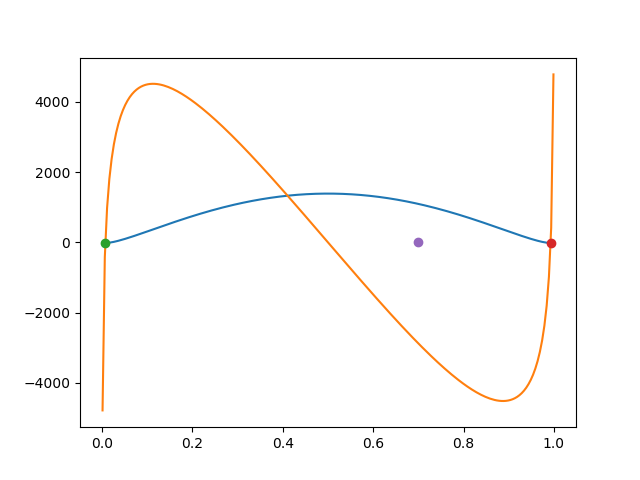
\includegraphics[width=.9\linewidth]{./mixture.png}
\end{center}

\begin{verbatim}
0.00718806418267 0.992811935817
\end{verbatim}

\section{Funny phase diagrams}
\label{sec:org3f854a7}
While \(\chi_\text{AB} \propto 1/T\) is the normal behavior, other dependencies are possible.

\begin{enumerate}
\item Construct a temperature vs.~composition diagram for a system for which
\(\chi_\text{AB}\) is a positive constant independent of temperature.

\item Construct a temperature vs.~composition diagram for a system for which
\(\chi_\text{AB} \propto T\).
\end{enumerate}

\subsection{Solution}
\label{sec:org042886b}
\begin{minted}[frame=lines,fontsize=\scriptsize,linenos]{python}
import numpy as np
import matplotlib.pyplot as plt
import scipy.optimize as opt

# free energy of mixing
def deltaf(xb):
    return R * T * ( xb * np.log(xb) + (1-xb) * np.log(1-xb)  + chi * xb * (1.-xb))

# first derivative
def ddeltaf(xb):
    return R * T * (np.log(xb) - np.log(1-xb) + chi * (1. - 2. * xb))

R = 8.314
chi = 2.5

xb = np.linspace(0.001,0.999,num=200)

plt.figure()
for T in [100,200,300,400,500]:
   plt.plot(xb,deltaf(xb),label=T)

plt.legend()
plt.savefig('ConstantComp.png')

plt.figure()
for T in [100,200,300,400,500]:
   chi = (T/100.) * 0.25 * 2.5
   plt.plot(xb,deltaf(xb),label=T)

plt.legend()
plt.savefig('Inverse.png')
\end{minted}

\begin{center}
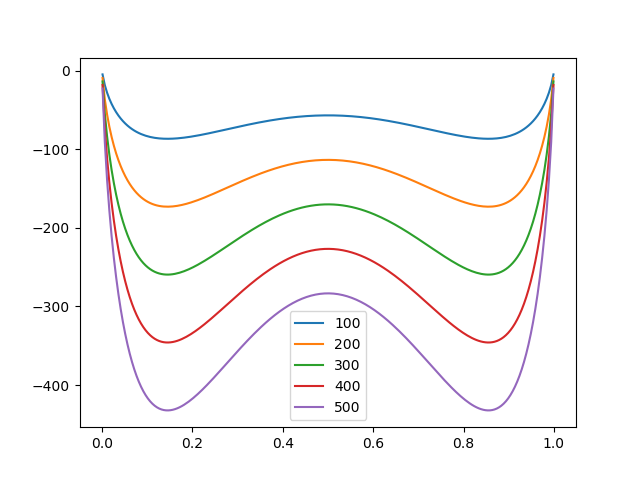
\includegraphics[width=.9\linewidth]{./ConstantComp.png}
\end{center}

\begin{center}
\includegraphics[width=.9\linewidth]{./inverse.png}
\end{center}

\section{Two components, two phases, too much fun!}
\label{sec:org2577332}
At \SI{300}{K}, the saturation pressure of A is ten times the saturation pressure of B. A and B mix ideally.

\begin{enumerate}
\item Write down an expression for the free energy of a two-component ideal liquid mixture as
a function of pressure and composition, \(g^{l}(P,x_{B})\).
\item Write down an expression for the free energy of a two-component ideal gas mixture as a
function of pressure and composition, \(g^{v}(P,y_{B})\).
\item Plot \(g^{l}\) and \(g^{v}\) vs composition at five pressure from \(P = P^{sat,B}\) to
\(P = P^{sat,A}\).  Identify the important regions on each plot.
\end{enumerate}

\subsection{solution}
\label{sec:org86cef3b}
\begin{minted}[frame=lines,fontsize=\scriptsize,linenos]{python}
import numpy as np
import matplotlib.pyplot as plt
from mpl_toolkits.mplot3d import Axes3D

def mu(mu0,x):
    return mu0 + RT * np.log(x)

# We are free to set chemical potential scale for A and B.
# Let chemical potentials of pure liquid A and B be 0. Can be any numbers
muAl0 = 0
muBl0 = 0

RT = 8.314*300
PBsat = 1
PAsat = 10

#P = np.linspace(PBsat,PAsat,num=10)
xB = np.linspace(0.01,0.99,num=20)
yB = np.linspace(0.01,0.99,num=20)

gl = (1-xB) * mu(muAl0,(1-xB)) + xB * mu(muBl0,xB)
for i in range(5):
   plt.subplot(5,1,i+1)
   P = PBsat + i*(PAsat-PBsat)/4.
   muAv0 = muAl0 + RT * np.log(P/PAsat)
   muBv0 = muBl0 + RT * np.log(P/PBsat)
   gv = (1-yB) * mu(muAv0,(1-yB)) + yB * mu(muBv0,yB)
   plt.plot(xB,gl)
   plt.plot(yB,gv)

plt.savefig('2phase.png')
\end{minted}

\begin{center}
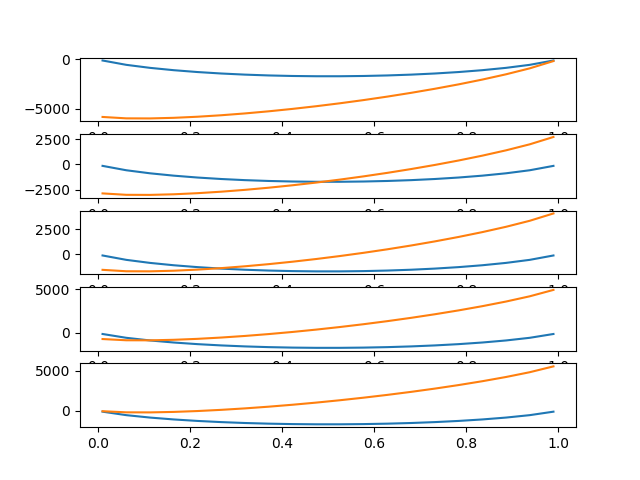
\includegraphics[width=.9\linewidth]{./2phase.png}
\end{center}

\section{Vapor-liquid equilibrium.}
\label{sec:orgea8202e}
The partial pressure of \ce{CS2} above a
  \ce{CS2}/dimethoxymethane (DMM) mixture at \(35.2^\circ\)C can be fit to the equation:
\begin{equation*}
  P_{\ce{CS2}} = x_{\ce{CS2}} (514.5~\text{torr}) \exp ( 1.4967 x_{\text{DMM}}^2 - 0.68175 x_{\text{DMM}}^3)
\end{equation*}

\begin{enumerate}
\item Use the Gibbs-Duhem relation to determine the partial pressure of DMM as a
function of composition.  Assume the vapor is ideal.
\item Do \ce{CS2} and DMM form a regular solution at these conditions?  \emph{Hint}: Determine the activities of each component and from these the excess free energy of mixing.  Is it proportional to \(x(1-x)\)?
\end{enumerate}

\subsection{Solution}
\label{sec:orgca60c05}
\begin{center}
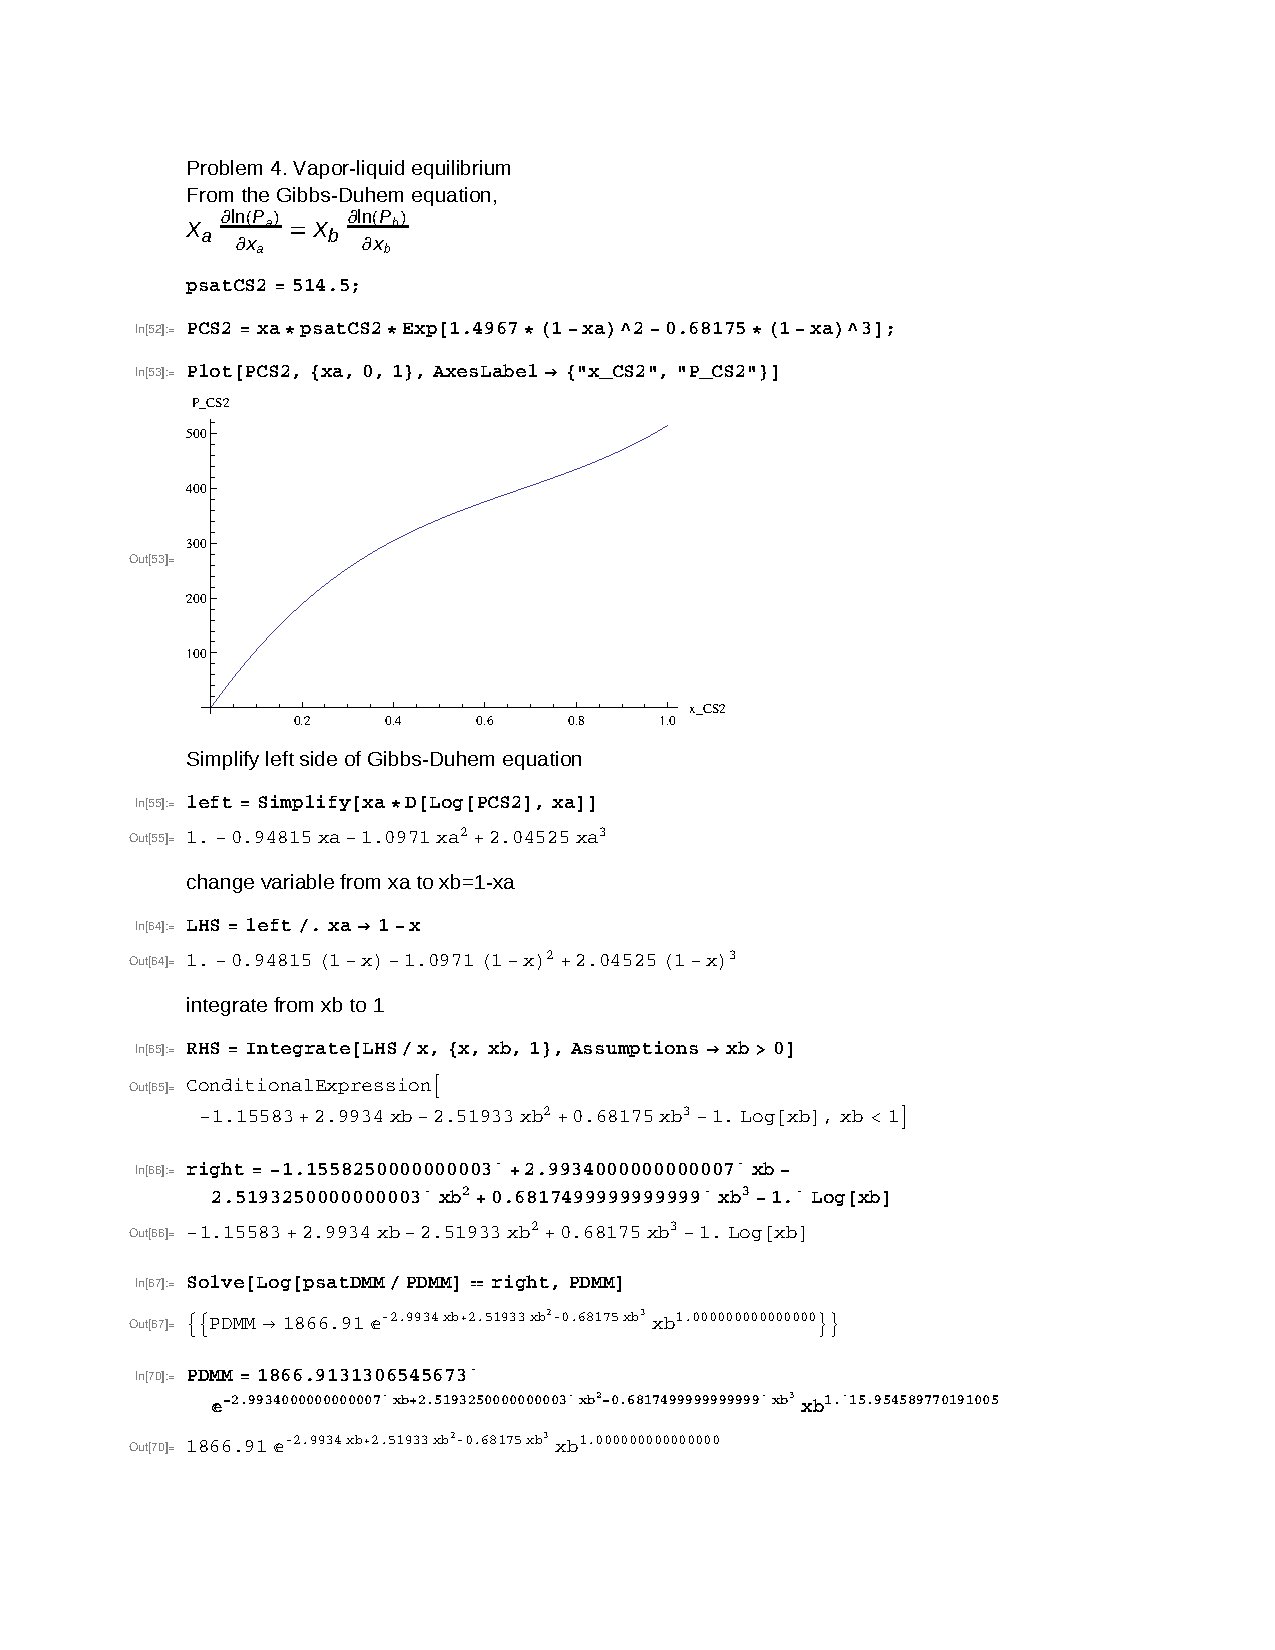
\includegraphics[width=.9\linewidth]{./HW8-Q4-soln.pdf}
\end{center}
\end{document}